% Installation of ug4 and introduction to its archtecture

\documentclass[xcolor=dvipsnames]{beamer}

\usepackage[latin1]{inputenc}
\usepackage{amsmath, amsfonts, amssymb}
\usepackage{graphicx}
\usepackage{color}
\usepackage{setspace}

\usetheme{Copenhagen}
\usecolortheme[named=YellowOrange]{structure}

%\usefonttheme{default}
\usefonttheme {structurebold}
\useinnertheme{default}
\useoutertheme{default}
\setbeamertemplate{headline}[default]

\newcommand*\oldmacro{}%
\let\oldmacro\insertshorttitle%
\renewcommand*\insertshorttitle{%
  \oldmacro\hfill%
  \insertframenumber\,/\,\inserttotalframenumber}

\title
 [ug4: Installation + Architecture]
 {ug4 simulation software toolbox: \\ Installation and Architecture}
\author [D. Logashenko] {Dmitry Logashenko}
\institute [CEMSE]
{CEMSE, KAUST, Saudi Arabia}
\date [Feb. 2025] {February 2025}

\begin{document}

\frame {\titlepage}

\begin {frame} [t]
\frametitle {Contents}
\tableofcontents
\end {frame}

\section {About ug4}

\begin {frame} [t]
\frametitle {ug4 toolkit}
\vspace {-2ex}
\begin {itemize}
	\item is a simulation software toolkit for {\color{blue} PDEs in 1d - 3d}
	\pause
	\item supports complicated geometries by {\color{blue} unstructured discretization grids}
		(ug = ``unstructured grids'')
	\pause
	\item implements a number of {\color{blue} efficient numerical methods} (discretizations, solvers,
		time-stepping schemes etc.) using the object oriented programming technology
	\pause
	\item supports {\color{blue} systems of PDEs} and contains built-in tools for different
		{\color{blue} coupling} techniques for the equations
	\pause
	\item has the MPI-based {\color{blue} parallelization}
	\pause
	\item provides a {\color{blue} plugin-based mechanism for extensions}
	\pause
	\item has built-in {\color{blue} VTK output}
	\pause
	\item includes a binding mechanism (e.g. for LUA {\color{blue} shell} and Python)
\end {itemize}
\pause
\begin {center}
\textbf {Therefore, ug4 presents a powerful tool for simulations with PDE based models, as well as
a researcher's construction kit for development and tests of numerical methods.}
\end {center}
\end {frame}

\begin {frame} [t]
\frametitle {Origination and technical info:}
\begin {itemize}
	\item Originally developed in the Goethe Center for Scientific Computing (Prof. Dr. G. Wittum),
	Frankfurt University.
	\pause
	\item Implemented in C++ (2011 standard).
	\pause
	\item Open-source and cross-platform.
	\pause
	\item Main parts and plugins are published in GitHub: https://github.com/UG4
	\pause
	\item ProMesh --- the ug4 GUI geometry handling tool: https://github.com/UG4/ProMesh
	\pause
	\item License: GNU Lesser General Public License version 3 with the additional requirements
		of explicit references to ug4 (in particular, in the bibliography).
	\pause
	\item Doxygen documentation, s. https://ug4.github.io/docs/index.html
\end {itemize}
\end {frame}

\section {Installation}

\begin {frame} [t]
\frametitle {Get ug4}
\vspace {-2ex}
\begin {itemize}
	\item Decide where you want to place it: \\
		{\color{blue} mkdir myUG4; cd myUG4}
	\pause
	\item Get ughub from github: \\
		{\color{blue} git clone https://github.com/UG4/ughub}
	\pause
	\item Create and initialize a directory for the source code \\
		{\color{blue} mkdir ug4; cd ug4}
	\pause
	\item Initialize this directory \\
		{\color{blue} ../ughub/ughub init}
	\pause
	\item Get the packages (the main library, plugins and applications) \\
		{\color{blue} ../ughub/ughub install Examples} \\
		This downloads not only the `Examples' package but also all its prerequisites
\end {itemize}
\end {frame}

\begin {frame} [t]
\frametitle {Configure the build system and build}
\vspace {-2ex}
\begin {itemize}
	\item ug4 uses Kitware {\color{blue} CMake} the build configuration (https://cmake.org/)
	\pause
	\item Return to the main directory (myUG4): \\
		{\color{blue} cd ..}
	\pause
	\item Create the build directory \\
		{\color{blue} mkdir build; cd build}
	\pause
	\item Initialize this directory, set the build options (s. below): \\
		{\color{blue} cmake ../ug4 -DDIM=2 -DCPU=1 -DPARALLEL=OFF}
	\pause
	\item Activate plugins you need: \\
		{\color{blue} cmake ../ug4 -DConvectionDiffusion=ON}
	\pause
	\item Make it (consider the -j option if supported in your system): \\
		{\color{blue} make} \\
		{\tiny (When using Visual Studio under MS Windows, open the .sln file with VS and build Release;
		alternatively use nmake or ninja instead of Unix make. You need further cmake options,
		s. below.)}
	\pause
	\item Result: You have created ugshell in myUG4/ug4/bin.
\end {itemize}
\end {frame}

\begin {frame} [t]
\frametitle {ug4 build options}
\begin {itemize}
	\item {\color{blue} DIM} --- dimensionalities (only these are accepted in the binding)
	\pause
	\item {\color{blue} CPU} --- selects the CPU algebra library and specifies
 		number of values per grid object, e.g. vertex (this can be plugin specific).
	\pause
 	\item {\color{blue} PARALLEL} --- if to compile the parallel version (then you need MPI)
	\pause
 	\item \dots
\end {itemize}

\pause
\vspace {2ex}
{\tiny For Visual Studio under MS Windows you may need additional options: \\
{\color{blue}-DSTATIC\_BUILD=ON -DCMAKE\_BUILD\_TYPE=Release -DLAPACK=OFF -DBLAS=OFF -DEMBEDDED\_PLUGINS=ON}
}
\end {frame}

\begin {frame} [t]
\frametitle {Other tools you need}
\begin {itemize}
	\item {\color{blue} ProMesh} --- a geometry editing and meshing GUI tool for ug4. It shares
		the geometry library with ug4. The grids are saved in the XML-based ugx. In particular, ProMesh and ug4 support
		projectors for curly boundaries. The GUI is based on Qt.
	\pause
	\item A viewer for VTK files, for ex. Kitware {\color{blue} ParaView}
		or LLNL {\color{blue} VisIt} (both open-source, cross-platform). \\
		ParaView: https://www.paraview.org \\
		VisIt: https://wci.llnl.gov/simulation/computer-codes/visit
\end {itemize}
\end {frame}

\begin {frame} [t]
\frametitle {First run}
We test ugshell for the numerical solution of a 2d Laplace equation with the script laplace.lua
is located in myUG4/ug4/apps/Examples/laplace.lua.

\pause
\vspace {2ex}
\emph{
{\color{red} Note} that ugshell has to find your LUA scripts and the plugins. There are 3 ways
to specify the paths:
\begin {itemize}
	\item prepend the full path to ugshell in the command line,
	\item set the UG4\_ROOT variable to myUG4/ug4,
	\item use command line option -rootpath with the path to myUG4/ug4.
\end {itemize}
}

\pause
\vspace {2ex}
Go to the Examples application:
{\color{blue} cd ../ug4/apps/Examples} \\
\pause
Run
{\color{blue} ../../bin/ugshell -ex laplace.lua -dim 2} \\
\pause
Now the solution is written to {\color{blue} sol\_laplace\_2d.vtu}.
\end {frame}

\begin {frame} [t]
\frametitle {A 3d example: Electromagnetic heating}
The installation can be reconfigured and rebuilt any time:
\begin {itemize}
	\item Return to the build directory: \\
		{\color{blue} cd myUG4/build}
	\pause
	\item Add 3d, allow 2 dof's per grid object, enable the Electromagnetism plugin: \\
		{\color{blue} cmake ../ug4 -DDIM="2;3" -DCPU="1;2"} \\
		{\color{blue} cmake ../ug4 -DElectromagnetism=ON}
	\pause
	\item Rebuild: \\
		{\color{blue} make} \\
	\pause
	\item You are now ready to run simulations in 2d and 3d, with plugins ConvectionDiffusion
		and Electromagnetism: \\
		{\color{blue} cd ../ug4/apps/Examples} \\
		{\color{blue} ../../bin/ugshell -ex electromagnetism\_pan.lua}
	\pause
	\item Try finer grids (longer computation time!): \\
		{\color{blue} ../../bin/ugshell -ex electromagnetism\_pan.lua -numRefs 4}
\end {itemize}
\end {frame}

\begin {frame} [t]
\only<1>
{%
 \centerline{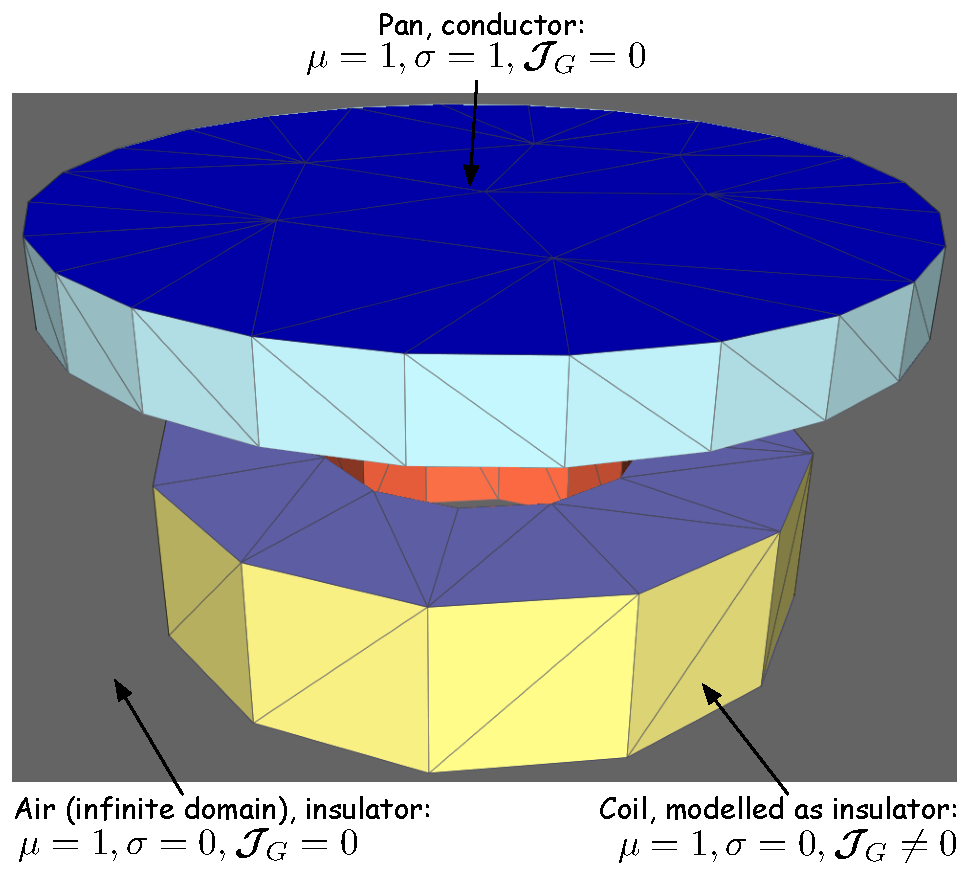
\includegraphics [width=0.9\textwidth] {coil_and_pan_v3_res.pdf}}
}
\only<2>
{%
 \centerline{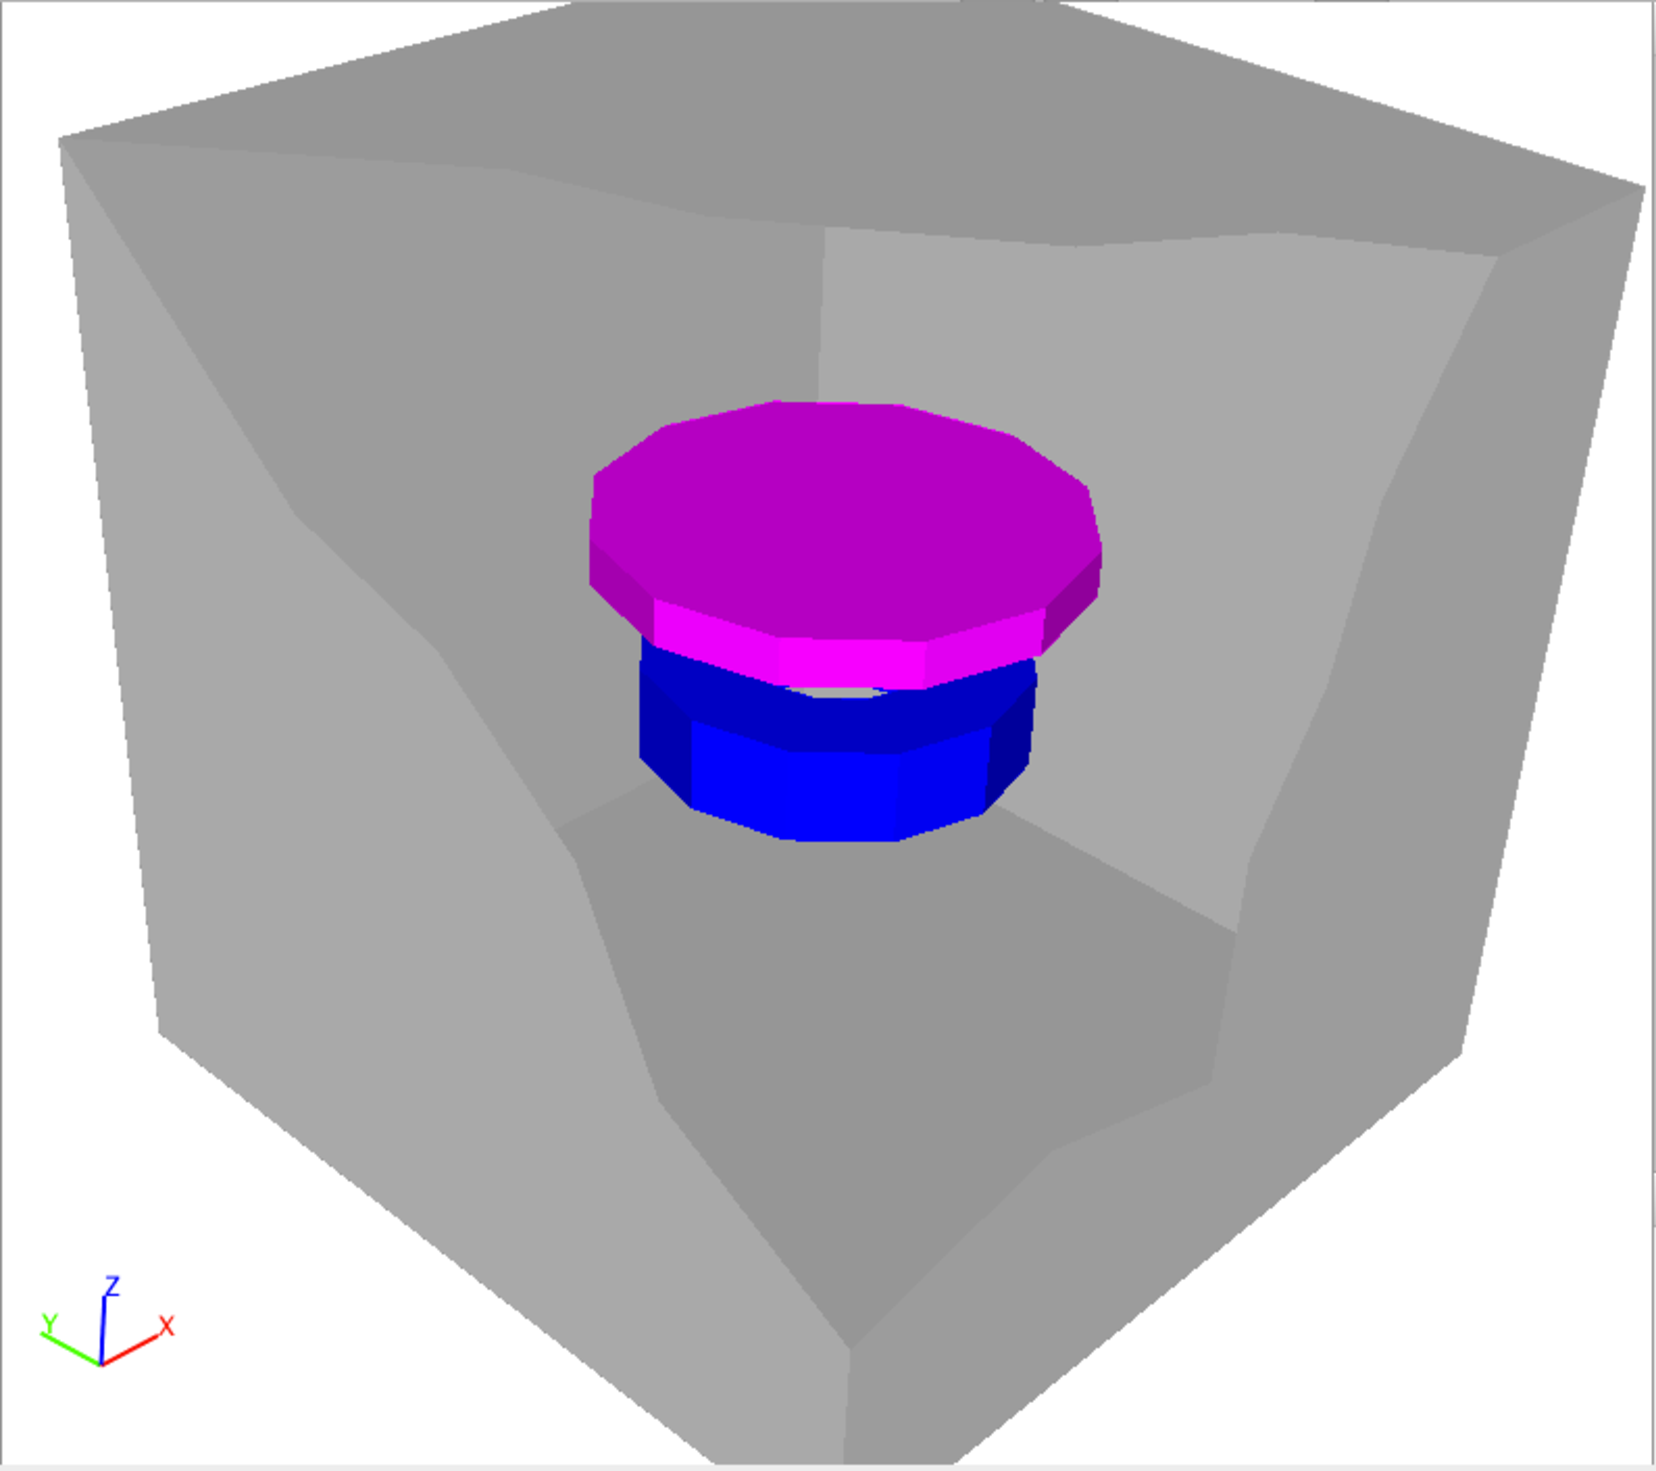
\includegraphics [width=0.9\textwidth] {Pan-Scheme.pdf}}
}
\only<3>
{%
 \centerline{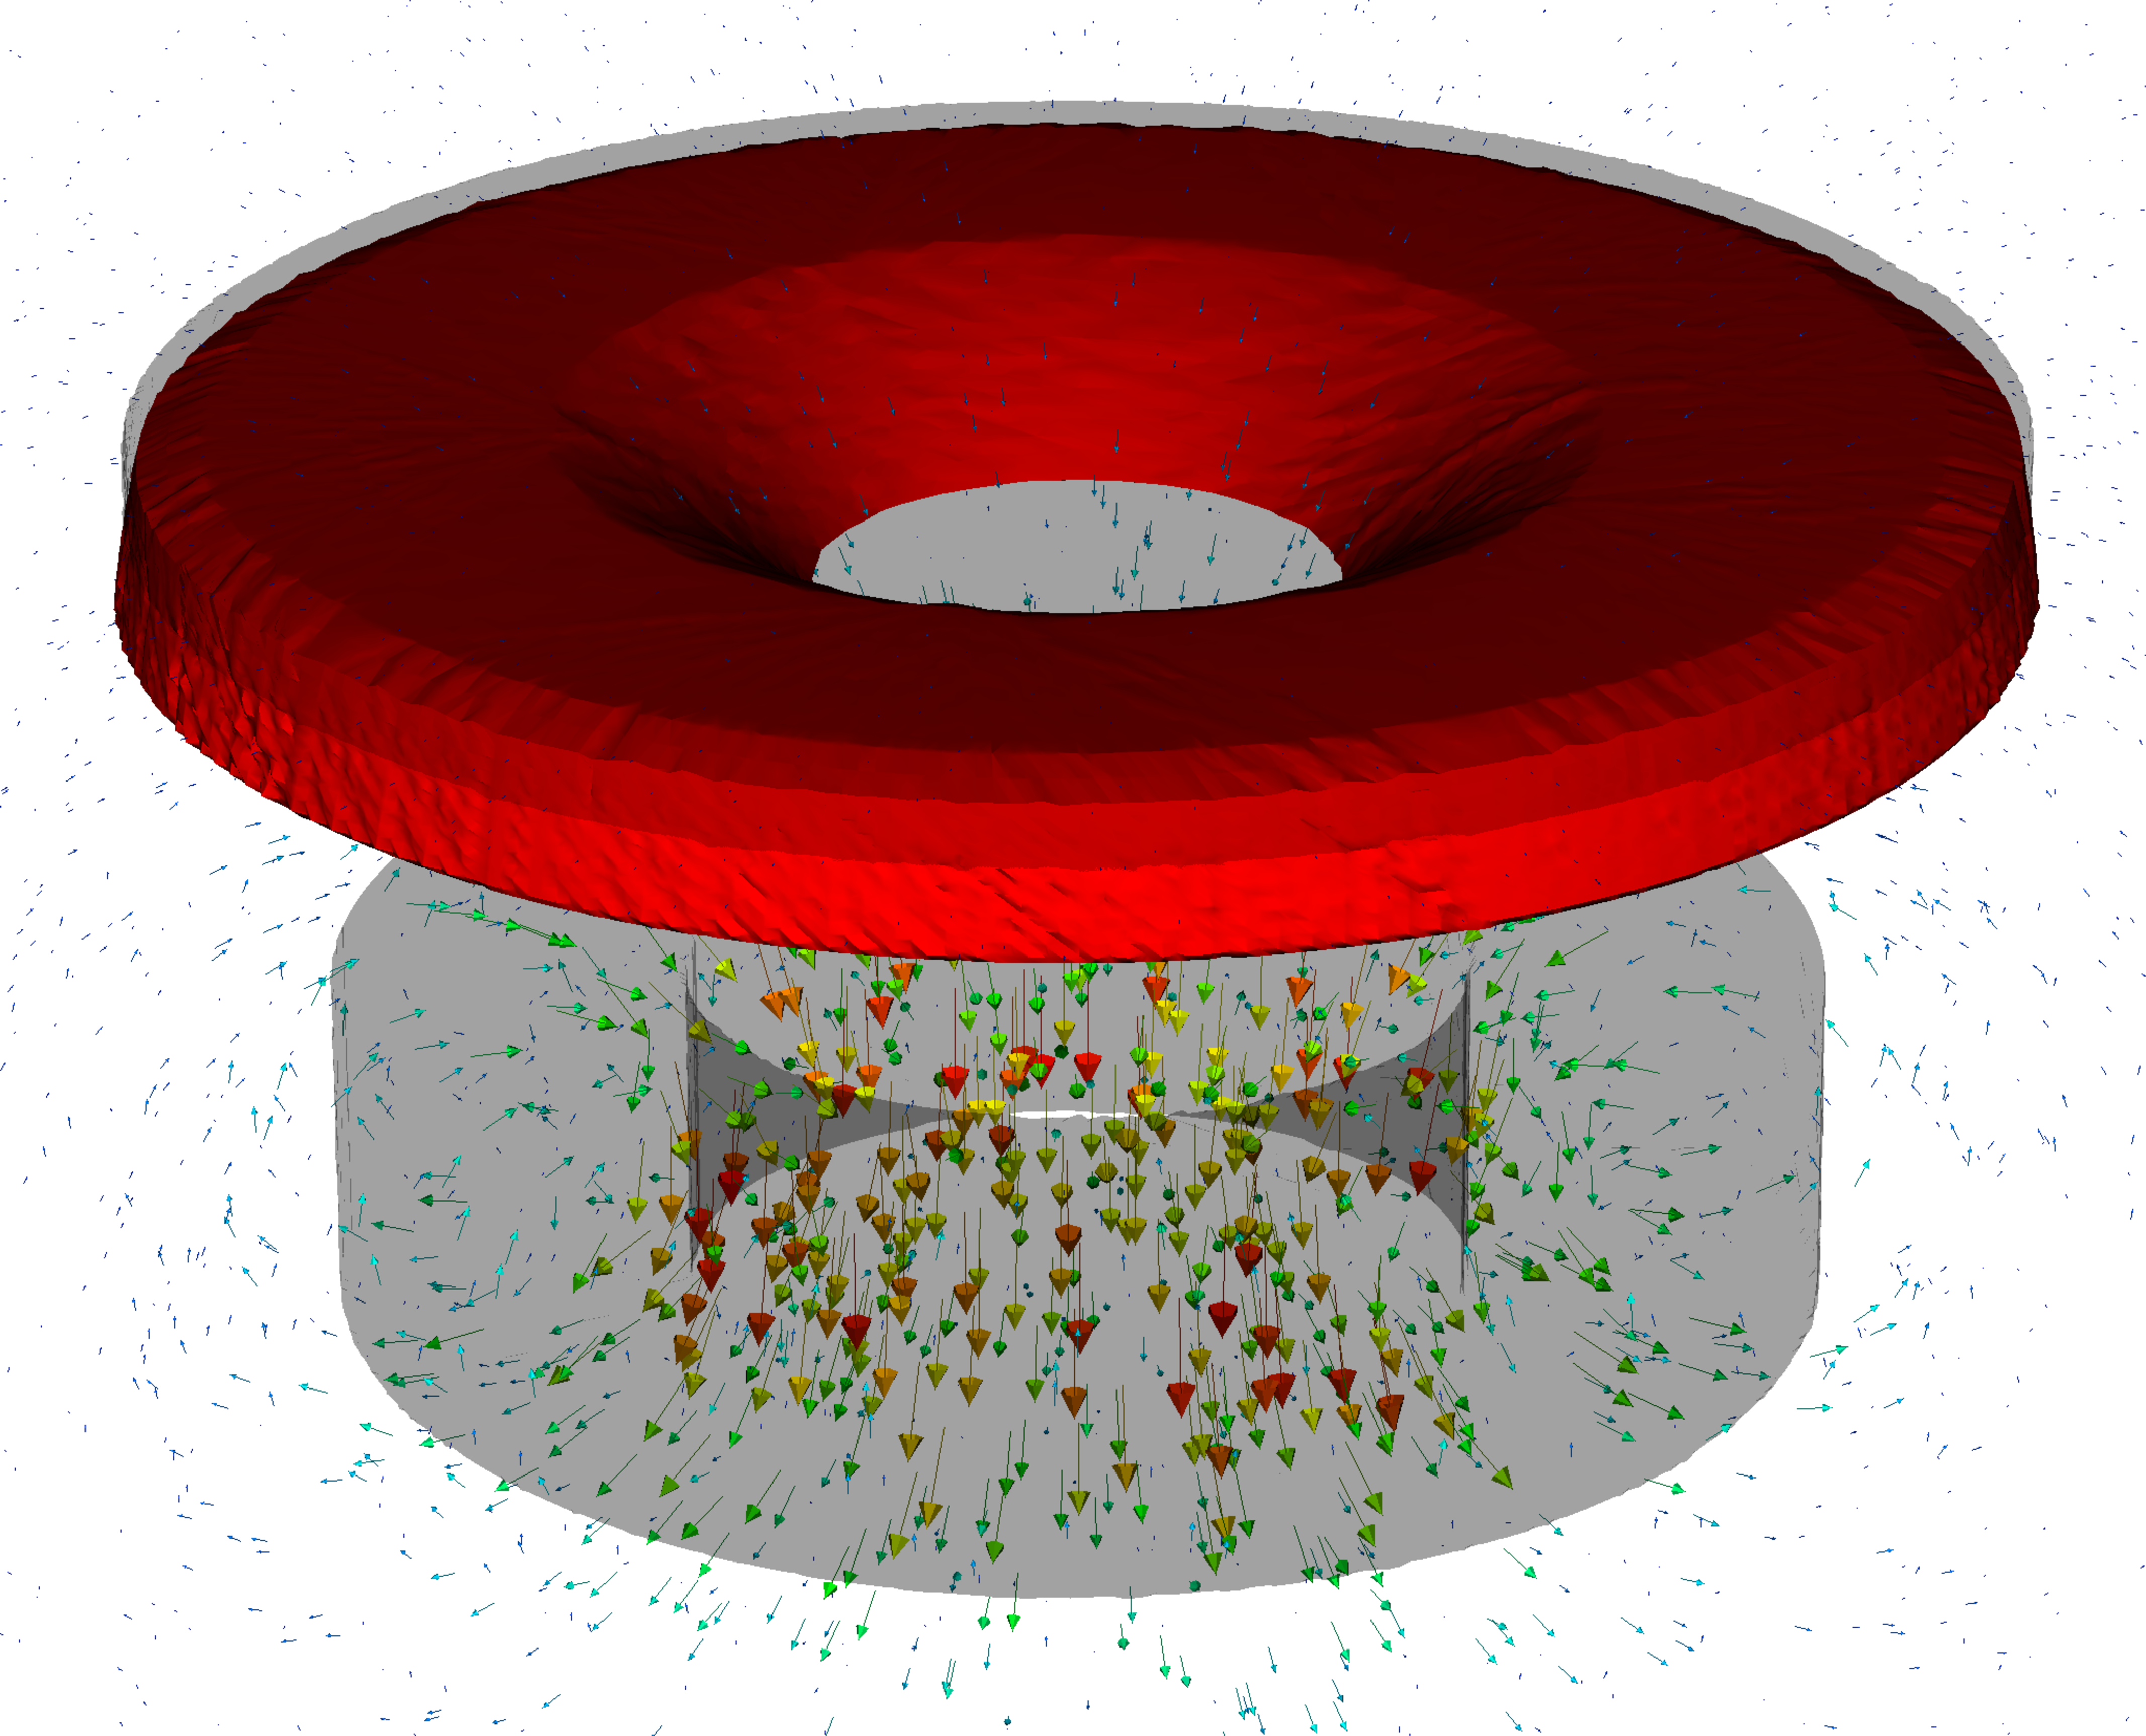
\includegraphics [width=0.9\textwidth] {PanSolution3d-coil_and_pan_v3-lev4.pdf}}
 \centerline{Arrows: $\mathrm{Re}\, \boldsymbol{\mathbf{B}}$, red: isosurfaces of the heat source.}
}
\end {frame}

\section {Architecture of ug4}

\begin {frame} [t]
\frametitle {ugcore, externals, plugins, applications and tools}
\vspace {-2ex}
\begin {itemize}
	\item ug4 is divided into several packages (separate git repos).
	\pause
	\item {\color{blue} ugcore} contains  main interface classes,  grid management modules,
		basic solvers, discretization utilities and output routines.
	\pause
	\item {\color{blue} plugins} are extensions of ugcore. After loading, their
		codes are indistinguishable from ugcore. Plugins implement local discretizations
		and model- or project-specific methods.
	\pause
	\item {\color{blue} externals} are 3rd party libraries used in ug4
	\pause
	\item {\color{blue} apps} (applications) are directories with grids (ugx-files), scripts etc.
	\pause
	\item {\color{blue} tools} are additional packages that do not depend on ugcore and are used for ex.
		for debugging.
\end {itemize}

\pause
\centerline {To get the list of the ug4 packages in github, run {\color{blue} ughub list}}

\pause
\centerline {Any user can {\color{blue} locally} add his own plugins, apps etc.}
\end {frame}

\begin {frame} [t]
\frametitle {ugcore libraries}
\vspace {-2ex}
\begin {itemize}
	\item ugcore consists of 3 main libraries: lib\_grid, lib\_algebra and lib\_disc.
	\pause
	\item {\color{blue} lib\_grid} implements the management of the geometry and the topology of the grid.
	\pause
	\item {\color{blue} lib\_algebra} provides the data structures for storing the grid functions and
		linear operators (represented by sparse matrices) without binding to the grid.
		It implements also basic geometry-independent linear solvers.
	\pause
	\item {\color{blue} lib\_disc} provides discretization tools and implements solvers that depend either
		on discretization interfaces or on the geometry. Furthermore, this library implements
		the coupling tools for discretizations.
	\pause
	\item Besides that, ugcore contains the {\color{blue} bridge} --- the interface to the
		scripting languages.
%	\pause
%	\item lib\_disc depends on lib\_grid and lib\_algebra, but lib\_grid and lib\_algebra are
%		completely independent on the other libraries.
\end {itemize}
\end {frame}

\begin {frame} [t]
\frametitle {Class templates: flexibility of the implementation}
\begin {itemize}
	\item ug4 C++ code is essentially based on {\color{blue} class templates}.
	\pause
	\item Implementation of most of the numerical methods depend on 2 template parameters:
		{\color{blue} TDomain} and {\color{blue} TAlgebra}. For that, implementation of this part can be replaced without
		reimplementing the method.
	\pause
	\item {\color{blue} TDomain} represents the grid, assignment of the degrees of freedom (DoFs) to the
		grid elements, type of the interpolation of the DoFs etc.
	\pause
	\item {\color{blue} TAlgebra} provides the storage for the DoFs and linear algebra.
	\pause
	\item Configuration parameters DIM and CPU determine the explicit instantiation of these templates in the bindings.
	\pause
	\item Templates and metaprogramming are also used in other parts of ug4 to achieve
		higher efficiency of the code.
\end {itemize}
\end {frame}

\section {Conclusions}

\begin {frame} [t]
\frametitle {Thank you for your attention!}
We considered:
\begin {itemize}
	\item Installation of ug4
	\item Demonstrative examples in 2d and 3d
	\item Architecture of ug4
\end {itemize}

\vspace{15ex}
{\tiny
References:
\begin {itemize}
	\item S. Reiter, A. Vogel, I. Heppner, M. Rupp, G. Wittum, A massively parallel geometric multigrid solver on hierarchically distributed grids, Computing and Visualization in Science 16(4), 2013, pp. 151--164, DOI: 10.1007/s00791-014-0231-x
	\item A. Vogel, S. Reiter, M. Rupp, A. N{\"a}gel, G. Wittum, UG 4: A novel flexible software system for simulating PDE based models on high performance computers, Computing and Visualization in Science 16(4), 2013, pp. 165--179, DOI: 10.1007/s00791-014-0232-9
\end {itemize}
}
\end {frame}

\end{document}

% End of File
